



\section{Introduction}
Sur l'ensemble des 35 probl\`emes, apr\`es avoir modifi\'e \`a la main les codes g\'en\'er\'es, seuls deux probl\`emes ne donnent
pas une valeur de Hessien correcte par {\it Tapenade}. Nous allons voir dans ce chapitre le temps d'ex\'ecution 
des d\'eriv\'ees et allons v\'erifier que les bornes th\'eoriques de complexit\'e sont respect\'ees. 
Ensuite, nous \'etudierons les variantes de m\'ethodes de descente sur la librairie MGH.


% \section{Temps de calcul des op\'erations critiques}
% Nous allons commencer par \'etudier les op\'erations \'el\'ementaires pour v\'erifier que les m\'ethodes sont comparables.
% Les tests ont \'et\'e effectu\'es sur des fonctions arbitrairement choisies.
% % 




\section{M\'ethode de descente avec recherche lin\'eaire}
Les m\'ethodes d'ordres sup\'erieurs requi\`erent souvent 
moins d'it\'erations. Nous pr\'esentons quelques exp\'eriences illustrant que notre implantation traduit cette r\'eduction du nombre
d'it\'erations dans une r\'eduction du temps de calcul. Les directions ont \'et\'e test\'ees avec et sans recherche lin\'eaire.
Il s'av\`ere que sans recherche lin\'eaire, les algorithmes n'aboutissent pas dans beaucoup de cas car $x_0$ est \'eloign\'e de la solution et
la direction peut être trop grande.
Pour les m\'ethodes de Newton et Chebychev, j'ai d'abord conserv\'e le point initial donn\'e dans les fonctions
de la librairie. Ce point est g\'en\'eralement assez proche de la solution. Dans le tableau, 
nous notons $x_{N_f}$ et $x_{C_f}$ les points finals des m\'ethodes de Newton et Chebychev respectivement. 
Cette norme confirme ou infirme le fait que les deux algorithmes convergent bien vers le même point.

On remarque sur la figure \ref{fig:vraies} que la m\'ethode de Chebychev comme celle d'extrapolation d'ordre trois,
 n'aboutit pas dans plusieurs cas, le maximum d'it\'erations \'etant fix\'e \`a $999$. Afin d'am\'eliorer ceci,
nous allons choisir la direction de Chebychev uniquement lorsqu'il s'agit bien d'une direction de descente.
 Dans le cas contraire nous reprendrons la direction de Newton.

% % Pourquoi n'est pas pertinent ?? On ne sais pas d\'ej\`a que les m\'ethodes convergent tr\`es mal 
% % a priori nous avons pas besoin de direction de descente -> 
% 
% \begin{table}%[h]
% 	\begin{center}
% 
% {\small
% \begin{tabular}{|l|c|c|c|c|c|c|}
%   \hline fonction & n & Iter Newton & Iter Cheb & temps Newton & temps Cheby & $\lVert x_{N_f}-x_{C_f}\rVert $\\
%  \hline
%    rose& $2$ & $22$ & $16$ & $0.020000$ & $0.016000$ & $0.000000$ \\\hline
%    froth& $2$ & $8$ & $6$ & $0.006000$ & $0.005000$ & $0.000000$ \\\hline
%    badscp& $2$ & $999$ & $999$ & $0.871000$ & $6.730000$ & $8.069786$ \\\hline
%    badscb& $2$ & $9$ & $999$ & $0.009000$ & $6.057000$ & $999792.981615$ \\\hline
%    beale& $2$ & $10$ & $999$ & $0.010000$ & $0.889000$ & $1043.480583$ \\\hline
%    jensam& $2$ & $11$ & $8$ & $0.010000$ & $0.007000$ & $0.000000$ \\\hline
%    helix& $3$ & $13$ & $14$ & $0.014000$ & $0.021000$ & $0.000000$ \\\hline
%    bard& $3$ & $13$ & $2$ & $0.013000$ & $0.003000$ & $Nan$ \\\hline
%    gauss& $3$ & $3$ & $3$ & $0.003000$ & $0.003000$ & $0.000000$ \\\hline
%    meyer& $3$ & $163^*$ & $13^*$ & $0.180000$ & $0.041000$ & $1.49\times 10^{10}$ \\\hline
%    gulf& $3$ & $2$ & $2$ & $0.003000$ & $0.027000$ & $Nan$ \\\hline
%    box& $3$ & $20$ & $999$ & $0.020000$ & $4.672000$ & $46.799375$ \\\hline
%    sing& $4$ & $22$ & $15$ & $0.020000$ & $0.013000$ & $0.000032$ \\\hline
%    wood& $4$ & $40$ & $29$ & $0.038000$ & $0.027000$ & $0.000000$ \\\hline
%    kowosb& $4$ & $9$ & $2$ & $0.009000$ & $0.003000$ & $Nan$ \\\hline
%    bd& $4$ & $9$ & $10$ & $0.008000$ & $0.009000$ & $0.000000$ \\\hline
%    rosex& $10$ & $22$ & $999$ & $0.021000$ & $4.290000$ & $2.837129$ \\\hline
%    singx& $12$ & $22$ & $17$ & $0.022000$ & $0.016000$ & $0.000134$ \\\hline
%    pen1& $4$ & $34$ & $999$ & $0.031000$ & $3.441000$ & $0.176609$ \\\hline
%    vardim& $10$ & $15$ & $11$ & $0.015000$ & $0.011000$ & $0.000000$ \\\hline
%    trig& $10$ & $10$ & $999$ & $0.012000$ & $1.080000$ & $2.883\times 10^{48}$ \\\hline
%    almost& $10$ & $9$ & $9$ & $0.008000$ & $0.010000$ & $0.214754$ \\\hline
%    bv& $10$ & $4$ & $3$ & $0.004000$ & $0.003000$ & $0.000000$ \\\hline
%    ie& $10$ & $4$ & $3$ & $0.004000$ & $0.003000$ & $0.000000$ \\\hline
%    band& $10$ & $9$ & $8$ & $0.009000$ & $0.008000$ & $0.000000$ \\\hline
%    cheb& $10$ & $18$ & $999$ & $0.025000$ & $5.302000$ & $0.235547$ \\\hline
%    \end{tabular}
% }
% 	\end{center}
% 	\label{tab:1}
% 	\caption{Tests des m\'ethodes de Newton et Chebychev sur l'ensemble de la librairie MGH avec $x_0$
% relativement proche de la solution. $Nb^*$ signifie que le crit\`ere d'Armijo plante.}
% 	\label{tab:newton}
% \end{table}










\begin{figure}
\caption{Profil des performances sur les fonctions de la librairie MGH, le point initial et les dimensions sont 
ceux par d\'efaut. Les m\'ethodes de Chebychev et Halley n'arrivent pas \`a la solution dans beaucoup de cas.}\center
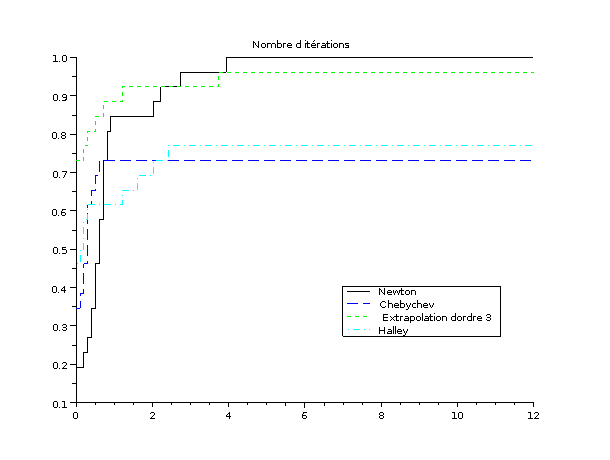
\includegraphics[scale=0.6]{figures/vraiesdirections.png}
\label{fig:vraies}
\end{figure}


L'utilisation de la direction de Newton lorsque celle de Chebychev n'est pas descendante am\'eliore significativement
l'algorithme. En revanche pour Halley, il n'y a presque pas de changement.
\begin{figure}
\caption{Profil des performances : les directions ne sont gard\'ees uniquement s'il s'agit de direction de descente, sinon on 
reprend celle de Newton. Cette fois-ci l'extrapolation d'ordre trois r\'eussit pour tous les probl\`emes.
}\center
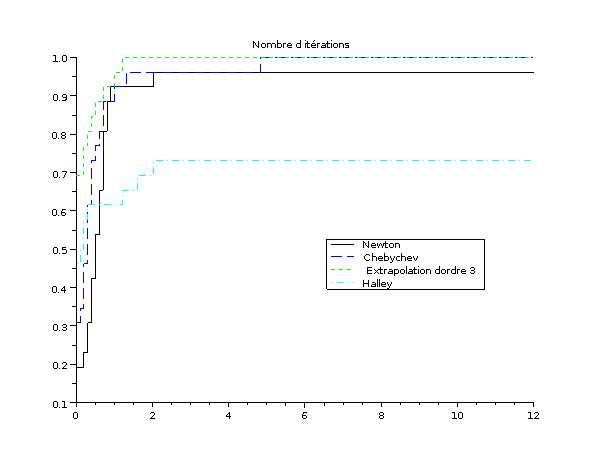
\includegraphics[scale=0.6]{figures/newtonquandpasdescendante.png}
\label{fig:dirnewton}
\end{figure}





% \begin{table}[h]
% 	\begin{center}
% {%\small
%  \footnotesize
% % ---------------------------------------sans l'extrapolation d'ordre 3
% % \begin{tabular}{|l|c|c|c|c|c|c|}
% %   \hline fonction & n & Iter Newton & Iter Cheb & temps Newton & temps Cheby &$\lVert x_{N_f}-x_{C_f}\rVert $\\
% %  \hline
% %    rose& $2$ & $22$ & $16$ & $0.020000$ & $0.017000$ & $0.000000$ \\\hline
% %    froth& $2$ & $8$ & $6$ & $0.007000$ & $0.005000$ & $0.000000$ \\\hline
% %    badscp& $2$ & $999$ & $545$ & $0.878000$ & $0.475000$ & $0.082534$ \\\hline
% %    badscb& $2$ & $9$ & $21$ & $0.009000$ & $0.037000$ & $0.000000$ \\\hline
% %    beale& $2$ & $10$ & $9$ & $0.011000$ & $0.011000$ & $0.000000$ \\\hline
% %    jensam& $2$ & $11$ & $8$ & $0.010000$ & $0.007000$ & $0.000000$ \\\hline
% %    helix& $3$ & $13$ & $14$ & $0.014000$ & $0.022000$ & $0.000000$ \\\hline
% %    bard& $3$ & $13$ & $13$ & $0.013000$ & $0.014000$ & $0.000000$ \\\hline
% %    gauss& $3$ & $3$ & $3$ & $0.003000$ & $0.003000$ & $0.000000$ \\\hline
% %    meyer& $3$ & $163^*$ & $133^*$ & $0.181000$ & $0.177000$ & $0.000000$ \\\hline
% %    gulf& $3$ & $2$ & $2$ & $0.003000$ & $0.004000$ & $Nan$ \\\hline
% %    box& $3$ & $20$ & $135$ & $0.020000$ & $0.132000$ & $66.947050$ \\\hline
% %    sing& $4$ & $22$ & $15$ & $0.020000$ & $0.013000$ & $0.000032$ \\\hline
% %    wood& $4$ & $40$ & $29$ & $0.038000$ & $0.027000$ & $0.000000$ \\\hline
% %    kowosb& $4$ & $9$ & $9$ & $0.009000$ & $0.009000$ & $0.000000$ \\\hline
% %    bd& $4$ & $9$ & $10$ & $0.009000$ & $0.009000$ & $0.000000$ \\\hline
% %    rosex& $10$ & $22$ & $20$ & $0.022000$ & $0.025000$ & $0.000000$ \\\hline
% %    singx& $12$ & $22$ & $17$ & $0.022000$ & $0.017000$ & $0.000134$ \\\hline
% %    pen1& $4$ & $34$ & $25$ & $0.031000$ & $0.023000$ & $0.000000$ \\\hline
% %    vardim& $10$ & $15$ & $11$ & $0.014000$ & $0.010000$ & $0.000000$ \\\hline
% %    trig& $10$ & $10$ & $9$ & $0.012000$ & $0.012000$ & $0.000000$ \\\hline
% %    almost& $10$ & $9$ & $9$ & $0.008000$ & $0.009000$ & $0.214754$ \\\hline
% %    bv& $10$ & $4$ & $3$ & $0.004000$ & $0.003000$ & $0.000000$ \\\hline
% %    ie& $10$ & $4$ & $3$ & $0.004000$ & $0.003000$ & $0.000000$ \\\hline
% %    band& $10$ & $9$ & $8$ & $0.009000$ & $0.008000$ & $0.000000$ \\\hline
% %    cheb& $10$ & $18$ & $20$ & $0.026000$ & $0.031000$ & $0.103538$ \\\hline
% %    \end{tabular}
% 
% \begin{tabular}{|l|c|c|c|c|c|c|c|c|c|}
%   \hline fonction & n & IN & IC & I3 & T N & T C& T E3 &  $\lVert x_{N_f}-x_{C_f}\rVert $ & $\lVert x_{N_f}-x_{3_f}\rVert $ \\
%  \hline
%    rose& $2$ & $22$ & $16$ & $15$ & $0.020$& $0.016$ & $0.019$  & $0.000000$ & $0.000000$ \\\hline
%    froth& $2$ & $8$ & $6$ & $5$ & $0.006$& $0.005$ & $0.005$  & $0.000000$ & $0.000000$ \\\hline
%    badscp& $2$ & $999$ & $545$ & $288$ & $0.874$& $0.477$ & $0.312$ & $0.082534$ & $0.235713$ \\\hline
%    badscb& $2$ & $9$ & $21$ & $18$ & $0.009$& $0.036$ & $0.075$ & $0.000000$ & $0.000000$ \\\hline
%    beale& $2$ & $10$ & $9$ & $8$ & $0.010$& $0.011$ & $0.020$ & $0.000000$ & $0.000000$ \\\hline
%    jensam& $2$ & $11$ & $8$ & $7$ & $0.009$& $0.007$ & $0.008$ & $0.000000$ & $0.000000$ \\\hline
%    helix& $3$ & $13$ & $14$ & $11$ & $0.013$& $0.022$ & $0.017$ & $0.000000$ & $0.000000$ \\\hline
%    bard& $3$ & $13$ & $13$ & $13$ & $0.013$& $0.014$ & $0.017$ & $0.000000$ & $0.000000$ \\\hline
%    gauss& $3$ & $3$ & $3$ & $3$ & $0.002$& $0.002$ & $0.003$ & $0.000000$ & $0.000000$ \\\hline
%    meyer& $3$ & $163^*$ & $133^*$ & $146^*$ & $0.196$& $0.184$ & $0.376$ & $0.000000$ & $0.000000$ \\\hline
%    gulf& $3$ & $2$ & $2$ & $2$ & $0.003$& $0.003$ & $0.010$ & $Nan$ & $Nan$ \\\hline
%    box& $3$ & $20$ & $135$ & $11$ & $0.020$& $0.131$ & $0.017$ & $66.947050$ & $0.000000$ \\\hline
%    sing& $4$ & $22$ & $15$ & $13$ & $0.020$& $0.014$ & $0.014$ & $0.000032$ & $0.000068$ \\\hline
%    wood& $4$ & $40$ & $29$ & $25$ & $0.038$& $0.027$ & $0.030$ & $0.000000$ & $0.000000$ \\\hline
%    kowosb& $4$ & $9$ & $9$ & $9$ & $0.010$& $0.009$ & $0.012$ & $0.000000$ & $0.000000$ \\\hline
%    bd& $4$ & $9$ & $10$ & $11$ & $0.008$& $0.009$ & $0.013$ & $0.000000$ & $0.000000$ \\\hline
%    rosex& $10$ & $22$ & $20$ & $13$ & $0.021$& $0.024$ & $0.023$ & $0.000000$ & $0.000000$ \\\hline
%    singx& $12$ & $22$ & $17$ & $16$ & $0.022$& $0.017$ & $0.020$ & $0.000134$ & $0.000155$ \\\hline
%    pen1& $4$ & $34$ & $25$ & $19$ & $0.031$& $0.023$ & $0.021$ & $0.000000$ & $0.000000$ \\\hline
%    vardim& $10$ & $15$ & $11$ & $10$ & $0.015$& $0.011$ & $0.012$ & $0.000000$ & $0.000000$ \\\hline
%    trig& $10$ & $10$ & $9$ & $9$ & $0.012$& $0.011$ & $0.017$ & $0.000000$ & $0.000000$ \\\hline
%    almost& $10$ & $9$ & $9$ & $12$ & $0.008$& $0.009$ & $0.020$ & $0.214754$ & $0.000000$ \\\hline
%    bv& $10$ & $4$ & $3$ & $3$ & $0.004$& $0.003$ & $0.004$ & $0.000000$ & $0.000000$ \\\hline
%    ie& $10$ & $4$ & $3$ & $3$ & $0.004$& $0.003$ & $0.003$ & $0.000000$ & $0.000000$ \\\hline
%    band& $10$ & $9$ & $8$ & $7$ & $0.009$& $0.008$ & $0.010$ & $0.000000$ & $0.000000$ \\\hline
%    cheb& $10$ & $18$ & $20$ & $13$ & $0.025$& $0.031$ & $0.039$ & $0.103538$ & $0.323658$ \\\hline
% 
% 
%    \end{tabular}
% }
% 	\end{center}
% 	\caption{Tests des m\'ethodes de Newton et Pseudo-Chebychev sur l'ensemble de la librairie MGH avec $x_0$
% relativement proche de la solution : pour Chebychev et l'extrapolation d'ordre 3 la direction n'est gard\'ee que s'il s'agit d'une 
% direction descendante sinon on reprend celle de Newton.}
% 	\label{tab:newton}
% \end{table}


Ensuite, j'ai effectu\'e les mêmes tests mais avec des dimensions plus grandes. Comme point de d\'epart,
j'ai d'abord choisi un nombre donn\'e par la fonction random, \`a valeurs comprises entre z\'ero et cent. Sachant que les algorithmes ne sont pas 
globalement convergents, le tableau \ref{tab:111} montre ce fait et en g\'en\'eral, ils ne convergent pas vers le même point.
Pour le tableau \ref{tab:dimplus}, j'ai choisi $1$, $10$ ou $100$ fois la valeur du point initial de la librairie MGH. Dans les cas o\`u 
les m\'ethodes convergent vers le même point, on peut noter une am\'elioration dans le nombre d'it\'erations. {\co
Pour la premi\`ere fonction du tableau, la diff\'erence des normes n'est pas \'egale mais les points finals obtenus ont un gradient v\'erifiant la condition
$\nabla f(x) \leq \epsilon$. L'\'ecart entre la valeur de l'objectif entre ces points est tr\`es faible. }
 En ce qui concerne le temps d'ex\'ecution,
il est meilleur pour Chebychev mais pour l'extrapolation d'ordre trois les temps sont moins bon car j'ai du partir du code fourni par le code des fonctions
car il n'est pas possible d'atteindre l'ordre $4$ avec Tapenade, même en essayant de modifier les routines PUSH et POP.
 



% \begin{table}%[h]
% 	\begin{center}
% {\small
% \begin{tabular}{|l|c|c|c|c|c|c|}
%   \hline fonction & $n$ & Iter Newton & Iter Cheb & temps Newton & temps Cheby & $\lVert x_{N_f}-x_{C_f}\rVert $ \\
%  \hline
% trig& $100 $&$ 6$ &$ 6 $&$ 0.072000 $&$ 0.056000 $&$ 0.000000$ \\\hline %en utilisant le x0
% ie& $300 $&$ 4 $&$ 3 $&$ 1.842000 $& $1.395000 $&$ 0.000000 $\\\hline % en utilisant le x0
% ie& $500 $&$ 4 $& $3 $& $8.047000$ &$ 6.110000 $&$ 0.000000$ \\\hline % en utilisant le x0
% ie& $800 $&$ 4 $& $3 $& $32.200000 $& $24.464000 $&$ 0.000000$ \\\hline % en utilisant le x0
% ie& $300 $&$ 7 $& $5 $& $3.204000$ & $2.324000$ & $0.000000$ \\\hline   % en utilisant le 10* x0
% ie& $500 $&$ 7 $& $5 $& $14.045000 $& $10.163000$ & $0.000000$ \\\hline % en utilisant le 10* x0
% ie& $800 $&$ 7 $&$ 5 $& $56.345000 $& $40.795000 $& $0.000000$ \\\hline % en utilisant le 10* x0
% band& $300$ &$ 9 $& $8$ &$ 0.352000 $& $0.345000 $& $0.000000 $\\\hline  % en utilisant le x0
% band& $500$ &$ 9 $& $8 $& $0.923000 $& $0.884000 $& $0.000000 $\\\hline  % en utilisant le x0
% band& $800$ &$ 9 $& $8 $& $2.566000 $& $2.450000 $& $0.000000 $\\\hline  % en utilisant le x0
% band& $300$ &$ 19$ & $15$ &$ 0.718000$ &$ 0.629000 $& $0.000000$ \\\hline
% \end{tabular}
% }
% 	\end{center}
% 	\caption{Point initial proche suffisamment proche de la solution pour que Chebychev converge : le gain en it\'eration
% n'est pas tr\`es grand. En revanche si la dimension est grande, le gain en temps peut être bon.}
% 	\label{tab:der}
% \end{table}

\begin{table}%[h]
	\begin{center}
{\small
\begin{tabular}{|l|c|c|c|c|c|c|c|c|c|c|}
  \hline fonction & $k*x_0$ & $n$ & IN & IC & I3 & TN & TC & T3 & $\lVert x_{N_f}-x_{C_f}\rVert $ & $\lVert x_{N_f}-x_{3_f}\rVert $  \\
 \hline
bv & 1 & 300 & 2 & 2 & 2 & 0.043 & 0.043 & 0.074 & 0.000042 & 0.000042 \\\hline 
bv & 10 & 300 & 4 & {\bf 3} & 4 & 0.082 & 0.065 & 0.149 & 0.000228 & 0.000308 \\\hline 
bv & 100 & 300 & 13 & {\bf 10 }& 11 & 0.266 & 0.218 & 0.413 & 0.000029 & 0.000267 \\\hline 
bv & 1 & 500 & 7 & 6 & {\bf 4} & 0.407 & 0.375 & 0.433 & 0.000725 & 0.000473 \\\hline 
bv & 10 & 500 & 13 & 13 & 15 & 0.747 & 0.815 & 1.626 & 0.001876 & 0.002417 \\\hline 
bv & 100 & 500 & 23 &{\bf 19} & 21 & 1.323 & 1.193 & 2.289 & 0.001084 & 0.000554 \\\hline 
bv & 1 & 800 & 6 & 5 &{\bf 3} & 1.062 & 0.942 & 0.920 & 0.016409 & 0.141987 \\\hline 
bv & 10 & 800 & 11 & 9 & {\bf 7} & 1.938 & 1.717 & 2.175 & 0.706669 & 0.924390 \\\hline 
bv & 100 & 800 & 21 &{\bf 20} & 17 & 3.720 & 3.841 & 5.325 & 0.798127 & 0.800345 \\\hline
ie & 1 & 300 & 4 & 3 & 3 & 1.834 & 1.398 & 1.468 & 0.000 & 0.000000 \\\hline 
ie & 10 & 300 & 7 & 5 & 5 & 3.205 & 2.330 & 2.474 & 0.000 & 0.000000 \\\hline 
ie & 1 & 500 & 4 & 3 & 3 & 8.044 & 6.105 & 6.348 & 0.000 & 0.000000 \\\hline 
ie & 10 & 500 & 7 & 5 & 5 & 14.054 & 10.155 & 10.556 & 0.000 & 0.000000 \\\hline 
ie & 1 & 800 & 4 & 3 & 3 & 32.521 & 24.463 & 25.169 & 0.000 & 0.000000 \\\hline 
ie & 10 & 800 & 7 & 5 & 5 & 56.313 & 40.456 & 41.555 & 0.000 & 0.000000 \\\hline 
trid & 1 & 300 & 7 & 6 & 6 & 0.152 & 0.129 & 0.204 & 0.000 & 0.000000 \\\hline 
trid & 10 & 300 & 12 & 10 & 10 & 0.246 & 0.215 & 0.344 & 0.000 & 0.000000 \\\hline 
trid & 100 & 300 & 18 & 15 & 14 & 0.369 & 0.325 & 0.482 & 0.000 & 0.000000 \\\hline 
trid & 1 & 500 & 7 & 6 & 6 & 0.397 & 0.366 & 0.579 & 0.000 & 0.000000 \\\hline 
trid & 10 & 500 & 12 & 10 & 10 & 0.673 & 0.613 & 0.967 & 0.000 & 0.000000 \\\hline 
trid & 100 & 500 & 18 & 15 &{\bf 14} & 1.015 & 0.906 & 1.333 & 0.000 & 0.000000 \\\hline 
trid & 1 & 800 & 7 & 6 & 6 & 1.177 & 1.080 & 1.656 & 0.000 & 0.000000 \\\hline 
trid & 10 & 800 & 12 & 10 & 10 & 2.043 & 1.842 & 2.757 & 0.000 & 0.000000 \\\hline 
trid & 100 & 800 & 18 & 15 & 14 & 3.067 & 2.760 & 3.854 & 0.000 & 0.000000 \\\hline 
band & 1 & 300 & 9 & 8 &{\bf 7} & 0.330 & 0.321 & 0.416 & 0.000 & 0.000000 \\\hline 
band & 10 & 300 & 19 & 15 & 15 & 0.695 & 0.608 & 0.894 & 0.000 & 0.000000 \\\hline 
band & 100 & 300 & 29 & 23 & 23 & 1.061 & 0.933 & 1.372 & 0.000 & 0.000000 \\\hline 
band & 1 & 500 & 9 & 8 &{\bf 7} & 0.904 & 0.895 & 1.149 & 0.000 & 0.000000 \\\hline 
band & 10 & 500 & 19 & 15 & 15 & 1.894 & 1.633 & 2.398 & 0.000 & 0.000000 \\\hline 
band & 100 & 500 & 29 & 23 & 23 & 2.892 & 2.508 & 3.680 & 0.000 & 0.000000 \\\hline 
band & 1 & 800 & 9 & 8 &{\bf 7} & 2.538 & 2.408 & 3.018 & 0.000 & 0.000000 \\\hline 
band & 10 & 800 & 19 & 15 & 15 & 5.391 & 4.570 & 6.468 & 0.000 & 0.000000 \\\hline 
band & 100 & 800 & 29 & 23 & 23 & 8.231 & 7.040 & 9.933 & 0.000 & 0.000000 \\\hline 
\end{tabular}
}
	\end{center}
	\caption{En testant avec des dimensions plus grandes. Comme point initial : 1, 10 ou 100 fois $x_0$. Le temps pour 
l'extrapolation d'odre 3 est plus grand car les d\'eriv\'ees sont calcul\'ees \`a partir du gradient fourni et non du mode inverse.
Les points finals de la premi\`ere fonction v\'erifient les conditions d'un gradient suffisamment petit.}
\label{tab:dimplus}


\end{table}

% \subsection{Avec r\'egion de confiance}
\subsection{Figures qui illustrent les parcours}


\paragraph{Rosenbrock}

Sur les figures \ref{fig:Newton} et \ref{fig:Chebychev}, j'ai trac\'e le chemin qu'emprunte 
l'algorithme de Newton et de Chebychev pour la fonction de Rosenbrock.
On observe bien que sans recherche lin\'eaire, l'algorithme est plus rapide,
cependant la valeur de l'objectif peut augmenter. \`A l'it\'eration $2$, la valeur de l'objectif
 atteint $1411.8$, et si l'algorithme revient vers la solution, c'est {$\scriptscriptstyle\ll$}par chance{$\scriptscriptstyle\gg$} car il n'y a pas de convergence globale.
 Lorsque l'on applique une recherche lin\'eaire, le parcours est mieux contrôl\'e et suit une {$\scriptscriptstyle\ll$}vall\'ee{$\scriptscriptstyle\gg$} o\`u la valeur de la
fonction objectif reste faible.

\begin{figure}
\caption{Newton - La recherche lin\'eaire restreint \`a fournir des it\'er\'es dont la valeur de l'objectif est 
toujours d\'ecroissante tandis que sans recherche, on s'\'eloigne pour converger plus vite.}
\begin{center}
\fbox{
\begin{minipage}[c]{0.6\textwidth}
\beginpgfgraphicnamed{figures/courbe_0}
\endpgfgraphicnamed \\
	  \begin{tabular}{|l|c|c|c|}
	  \hline
	  it\'eration & $x_1$ & $x_2$ &  $f(x)$ \\
	  \hline
	  $0$ & $-1.200000$ & $1.000000$ & $24.200000$ \\
	  $1$ & $-1.175281$ & $1.380674$ & $4.731884$ \\
	  $2$ & $0.763115$ & $-3.175034$ & $1411.845179$ \\
	  $3$ & $0.763430$ & $0.582825$ & $0.055966$ \\
	  $4$ & $0.999995$ & $0.944027$ & $0.313189$ \\
	  $5$ & $0.999996$ & $0.999991$ & $0.000000$ \\
	  $6$ & $1.000000$ & $1.000000$ & $0.000000$ \\
	  \hline
	  \end{tabular}\\
\end{minipage}
}
\end{center}
\label{fig:Newton}
\end{figure}

% \vspace{1cm}


% \begin{table}%[h]
% 	\begin{center}
% 	  \begin{tabular}{|l|c|c|c|}
% 	  \hline
% 	  it\'eration & $x_1$ & $x_2$ &  $f(x)$ \\
% 	  \hline
% 	  $0$ & $-1.200000$ & $1.000000$ & $24.200000$ \\
% 	  $1$ & $-1.175281$ & $1.380674$ & $4.731884$ \\
% 	  $2$ & $0.763115$ & $-3.175034$ & $1411.845179$ \\
% 	  $3$ & $0.763430$ & $0.582825$ & $0.055966$ \\
% 	  $4$ & $0.999995$ & $0.944027$ & $0.313189$ \\
% 	  $5$ & $0.999996$ & $0.999991$ & $0.000000$ \\
% 	  $6$ & $1.000000$ & $1.000000$ & $0.000000$ \\
% 	  \hline
% 	  \end{tabular}\\
% 	\end{center}
% 	\caption{It\'er\'es de la m\'ethode de Newton sur la fonction Rosenbrock sans recherche lin\'eaire.}
% 	\label{tab:newton}
% \end{table}





\begin{figure}
\caption{Chebychev - La direction de Chebychev est meilleure sur l'exemple, cependant qu'une seule it\'eration n'est gagn\'ee}
\begin{center}
\fbox{
\begin{minipage}[c]{0.6\textwidth}
% \begin{center}
\beginpgfgraphicnamed{figures/courbe_1}
\endpgfgraphicnamed \\
	\begin{tabular}{|l|c|c|c|}
	\hline
	it\'eration & $x_1$ & $x_2$ &  $f(x)$ \\
	\hline
	$0$ & $-1.200000$ & $1.000000$ & $24.200000$ \\
	$1$ & $-1.150840$ & $1.322626$ & $4.626437$ \\
	$2$ & $0.848588$ & $-0.780668$ & $225.254139$ \\
	$3$ & $0.849592$ & $0.721806$ & $0.022623$ \\
	$4$ & $1.000000$ & $0.999993$ & $0.000000$ \\
	$5$ & $1.000000$ & $1.000000$ & $0.000000$ \\
	\hline
	\end{tabular}
%\end{center}
\end{minipage}
}
\end{center}
% \beginpgfgraphicnamed{figures/courbe_1}
% \endpgfgraphicnamed

\label{fig:Chebychev}
\end{figure}


% \begin{table}%[h]
% 	\begin{center}
% 	\begin{tabular}{|l|c|c|c|}
% 	\hline
% 	it\'eration & $x_1$ & $x_2$ &  $f(x)$ \\
% 	\hline
% 	$0$ & $-1.200000$ & $1.000000$ & $24.200000$ \\
% 	$1$ & $-1.150840$ & $1.322626$ & $4.626437$ \\
% 	$2$ & $0.848588$ & $-0.780668$ & $225.254139$ \\
% 	$3$ & $0.849592$ & $0.721806$ & $0.022623$ \\
% 	$4$ & $1.000000$ & $0.999993$ & $0.000000$ \\
% 	$5$ & $1.000000$ & $1.000000$ & $0.000000$ \\
% 	\hline
% 	\end{tabular}
% 	\end{center}
% 	\caption{It\'er\'es de la m\'ethode de Chebychev sur la fonction Rosenbrock}
% 	\label{tab:chebychev}
% \end{table}




\begin{figure}%[!h]
\caption{Ordre sup\'erieur : la direction s'\'eloigne encore moins de la vall\'ee que les proc\'ed\'es de Newton ou Chebychev.}
\begin{center}
\fbox{
\begin{minipage}[c]{0.7\textwidth}
\beginpgfgraphicnamed{figures/courbe_2}
\endpgfgraphicnamed \\
	\begin{tabular}{|l|c|c|c|}
	\hline
	it\'eration & $x_1$ & $x_2$ &  $f(x)$ \\
	\hline
	$0$ & $-1.200000$ & $1.000000$ & $24.200000$ \\
	$1$ & $-1.126673$ & $1.265834$ & $4.524003$ \\
	$2$ & $0.847210$ & $-0.350714$ & $114.187943$ \\
	$3$ & $0.849335$ & $0.721366$ & $0.022700$ \\
	$4$ & $1.000000$ & $1.000000$ & $0.000000$ \\
	$5$ & $1.000000$ & $1.000000$ & $0.000000$ \\
	\hline
	\end{tabular}\\
\end{minipage}
}
\end{center}
\label{fig:sup}
\end{figure}





% \begin{table}%[!h]
% 	\begin{center}
% 	\begin{tabular}{|l|c|c|c|}
% 	\hline
% 	it\'eration & $x_1$ & $x_2$ &  $f(x)$ \\
% 	\hline
% 	$0$ & $-1.200000$ & $1.000000$ & $24.200000$ \\
% 	$1$ & $-1.126673$ & $1.265834$ & $4.524003$ \\
% 	$2$ & $0.847210$ & $-0.350714$ & $114.187943$ \\
% 	$3$ & $0.849335$ & $0.721366$ & $0.022700$ \\
% 	$4$ & $1.000000$ & $1.000000$ & $0.000000$ \\
% 	$5$ & $1.000000$ & $1.000000$ & $0.000000$ \\
% 	\hline
% 	\end{tabular}\\
% 	\end{center}
% 	\caption{It\'er\'es de la m\'ethode d'extrapolation d'ordre 3 sur la fonction Rosenbrock}
% 	\label{tab:extra3}
% \end{table}


% \cite{historical}\cite{cauchy}

{\co
\section{Conclusion}
Par l'interpr\'etation de ces r\'esultats, nous pouvons conclure qu'il est possible d'obtenir des m\'ethodes convergant plus rapidement
que la m\'ethode de Newton dans un cas g\'en\'eral. De plus, l'efficacit\'e est meilleure; les temps de calcul sont r\'eduits. Malheureusement,
la DA est encore immature pour fournir l'ordre 4 de mani\`ere efficace. On peut cependant esp\'erer que les outils de DA seront bientôt capable
d'atteindre ces ordres de d\'erivations de mani\`ere syst\'ematique. En ce sens, nous pourrons gagner du temps grâce au m\'ethodes d'ordre sup\'erieur
et ce, d'autant que la dimension du probl\`eme est grande.
}
